\documentclass[11pt,a4paper]{article}
\usepackage[utf8]{inputenc}
\usepackage[english]{babel}
\usepackage{amsmath,amssymb}
\usepackage{hyperref}
\usepackage{geometry}
\geometry{margin=2.5cm}
\usepackage{booktabs}
\usepackage{tikz}
\usetikzlibrary{shapes,arrows,positioning}

\title{The Ghost: an ephemeral inner-reasoning layer\\ \large Concept note and working prototype --- v0.01}
\author{dr.\ Francesco Bulla --- Bologna, 09/10/2026}
\date{Local draft, unpublished --- v0.01}

\begin{document}
\maketitle

\begin{abstract}
The Ghost is an inner-reasoning layer that activates before output generation,
produces a thought in a private numeric code, uses it to reformulate the request,
and then erases it. The user only sees the final output. This note collects the
original intuition (Catania, October 7 2026), three design decisions that make it
implementable, the \texttt{src/fantasma} prototype, and the first live experiments with
DeepSeek-V4.1-Flash (API id \texttt{deepseek-flash}). Four real-world cases and a code
test show the Ghost excels at framing and reformulating, while execution remains a
second step. The trade-off between cognitive privacy and verifiability is structural
and is made explicit, not hidden.
\end{abstract}

\section{Idea}
The Ghost emerges, acts, disappears. It leaves a trace only for whoever evoked it.
Unlike visible Chain-of-Thought, hidden scratchpads and latent reasoning, erasure here
is active and the code is private: a numeric sequence (e.g.\ \texttt{0984567345679})
uninterpretable from the outside.

\section{Mechanism}
\begin{enumerate}
\item Input reaches the model.
\item An internal gate decides whether to activate the Ghost.
\item The Ghost generates a private numeric thought.
\item The same model re-reads its own code (decision 5.1).
\item The reformulated input produces the final output.
\item The thought is erased; only a cryptographic commitment (hash) remains.
\end{enumerate}

\begin{figure}[h]
\centering
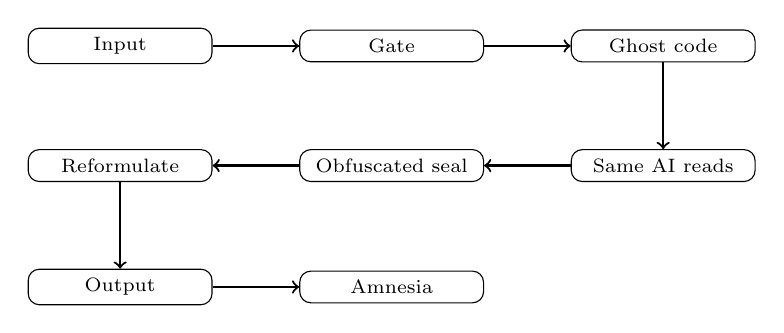
\begin{tikzpicture}[node distance=1.1cm, auto,
  blocco/.style={rectangle, draw, rounded corners, text width=2.1cm, align=center, font=\scriptsize},
  freccia/.style={->, thick}]
\node[blocco] (in) {Input};
\node[blocco, right=of in] (gate) {Gate};
\node[blocco, right=of gate] (ghost) {Ghost code};
\node[blocco, below=of ghost] (interp) {Same AI reads};
\node[blocco, left=of interp] (seal) {Obfuscated seal};
\node[blocco, left=of seal] (ref) {Reformulate};
\node[blocco, below=of ref] (out) {Output};
\node[blocco, right=of out] (amn) {Amnesia};
\draw[freccia] (in) -- (gate);
\draw[freccia] (gate) -- (ghost);
\draw[freccia] (ghost) -- (interp);
\draw[freccia] (interp) -- (seal);
\draw[freccia] (seal) -- (ref);
\draw[freccia] (ref) -- (out);
\draw[freccia] (out) -- (amn);
\end{tikzpicture}
\caption{The Ghost cycle: emerge, act, disappear. Only the hash audit remains.}
\end{figure}

\section{Three design decisions}
\textbf{5.1 --- The same AI interprets.} No external decoder: the code is handed back
to the same model via a \texttt{FANTASMA-INTERPRETA} prompt. Only that state, in that
turn, can read it. Without salt and nonce it cannot be reconstructed.

\textbf{5.2 --- Obfuscated cache.} The raw code lives in ephemeral memory only for the
interpretation turn. It is then sealed into cache in obfuscated form (digit shift derived
from the salt, i.e.\ the AI's inner state). The cache never holds the raw; with the wrong
salt one gets noise.

\textbf{5.3 --- Amnesia after output.} Once the output is out, there is nothing to remember.
Ephemeral memory and cache are wiped. No persistent vector store. Only the hash-chained
audit remains, recording commitments, never contents.

\section{Prototype}
\texttt{src/fantasma}: \texttt{gate.py} (inspectable heuristic gate),
\texttt{codec.py} (HMAC + nonce, every Ghost unique),
\texttt{memory.py} (\texttt{EphemeralMemory} + \texttt{ObfuscatedCache}),
\texttt{audit.py} (content-free hash chain),
\texttt{pipeline.py} (1--8 flow),
\texttt{llm\_deepseek.py} (DeepSeek-V4.1-Flash adapter, key from env only).
Suite: 12 tests green locally and on Docker (\texttt{docker run --rm fantasma:0.1}).

\section{Live experiments (09/10/2026)}
Model: DeepSeek-V4.1-Flash (\texttt{deepseek-flash}), \texttt{reasoning\_effort=high},
\texttt{thinking=enabled}. All cases: ghost on, same-AI on, memory and cache empty
afterwards, audit verified.

\begin{center}
\begin{tabular}{lll}
\toprule
Case & Reformulation & Output \\
\midrule
Milan/Catania decision & values and constraints made explicit & clarified question \\
Message to collaborator & firm-professional tone & ready-to-send draft \\
Web-app brief & phases, alternatives, risks & operational question \\
Ethical paradox & procedural conditions & thesis: consent and contestability \\
Code test & 4 bugs identified & analysis + fix in 2 steps \\
\bottomrule
\end{tabular}
\end{center}

On code the Ghost found every hidden flaw (mutable default, \texttt{range(len+1)},
division by zero, misleading names), produced an executable specification and, at the
second step, 391 lines of implementation with tests. First run red on one over-strict
assert (extra keys), then green after a one-line fix: \texttt{Tutti i test sono passati.}

\section{Open problems and the ethical paradox}
What remains: grounding a private language (Wittgenstein), causal erasure being
impossible in a transformer, learning without persistent memory, auditing without
revealing. The principle ``no one shall decide how someone else reasons'' stays in
tension with gate, code and erasure being designed: the gate is therefore explicit and
configurable, never hidden. The privacy--verifiability trade-off is structural.

\begin{figure}[h]
\centering
\begin{tikzpicture}[font=\scriptsize]
\draw[->] (0,0) -- (7,0) node[right] {cognitive privacy};
\draw[->] (0,0) -- (0,4) node[above] {verifiability};
\draw[thick] (0.5,3.5) .. controls (3,3) and (4,1) .. (6.5,0.5);
\fill (0.7,3.4) circle (2pt) node[above right] {visible CoT};
\fill (3.4,2.0) circle (2pt) node[above right] {Ghost};
\fill (6.2,0.6) circle (2pt) node[above] {black box};
\end{tikzpicture}
\caption{The more private the thought, the less verifiable. The Ghost sits in the middle, declared.}
\end{figure}

\section{Vision}
The Ghost does not aim at a more opaque model, but at a legitimate, procedural opacity:
consent, contestability, time bounds, independent gate oversight.

\begin{figure}[h]
\centering
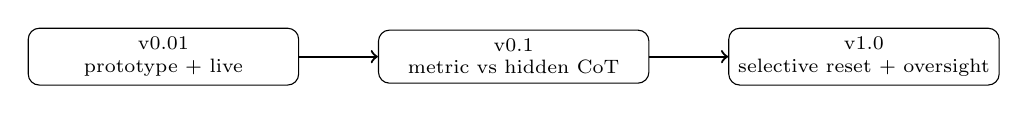
\begin{tikzpicture}[font=\scriptsize,
  tappa/.style={rectangle, draw, rounded corners, align=center, text width=3.2cm}]
\node[tappa] (v1) {v0.01 \\ prototype + live};
\node[tappa, right=1cm of v1] (v2) {v0.1 \\ metric vs hidden CoT};
\node[tappa, right=1cm of v2] (v3) {v1.0 \\ selective reset + oversight};
\draw[->, thick] (v1) -- (v2);
\draw[->, thick] (v2) -- (v3);
\end{tikzpicture}
\caption{Roadmap: from a working prototype to measurement, then to guarantees.}
\end{figure}

\section{Status and next steps}
Status: concept + working v0.01 prototype, 12 green tests, recorded live experiments.
Next: measurable improvement metric vs.\ hidden CoT, true selective reset, independent
gate oversight. Otherwise it stays in the notebook: not every idea must become a paper;
some are just beautiful. This one, for now, works.
\end{document}
